\chapter{Implementación  \textit{hardware} }

Para implementar el algoritmo en  \textit{hardware}  dividimos en módulos el algoritmo de filtrado, el algoritmo
de detección de picos y el algoritmo de detección de arritmias, estos los unificamos en un módulo principal 
y probamos la simulación con un \textit{testbench}. Véase \Cref{fig:diagramaGeneral}

\begin{figure}[h!]
    \centering
    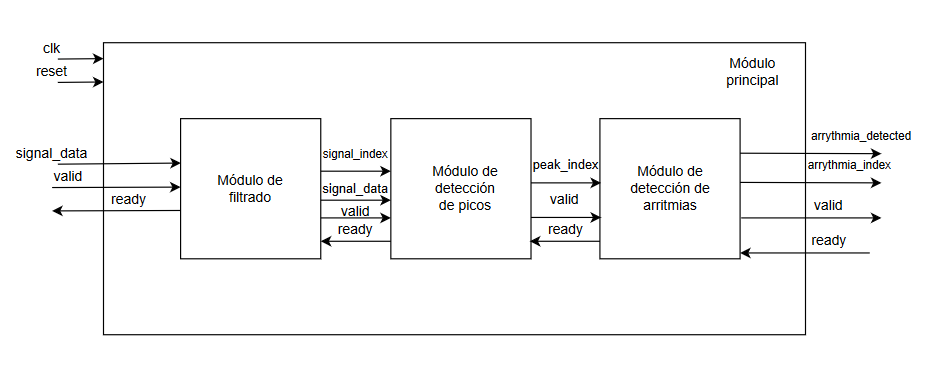
\includegraphics[width=0.99\textwidth]{./Images/img_res_experimentales/diagramaGeneral.png}
    \caption{Diagrama principal de todos los módulos a evaluar}
    \label{fig:diagramaGeneral}
\end{figure} 




\section{Módulos adicionales} 

Como los valores de las señales están en punto flotante y como se necesitan almacenar valores en una memoria, para poder operar con ellos, es necesario utilizar módulos  \textit{hardware}  que permitan hacer dichas operaciones. Para ello, se utilizarán los \textit{IP cores} (\textit{Intelectual Property cores}) de Vivado \cite{xilinx_ip_cores}. Estos \textit{IP cores} son bloques que pueden realizar funciones específicas de  \textit{hardware} , optimizando así el diseño y facilitando la implementación de operaciones complejas. En este proyecto utilizaremos módulos de multiplicación y suma, resta, división y comparación de números en punto flotante, aprovechando las capacidades de los \textit{IP cores} de Vivado para manejar estos cálculos de manera eficiente y precisa.
\subsection{Módulos ROM y RAM}
 Se necesitan módulos de ROM y RAM para las pruebas y para el módulo de filtrado.

 Para poder hacer una simulación, en la parte de las pruebas, se necesitan tres memorias ROM: Una para almacenar los valores de la señal original, otra para almacenar un bit que indique si se ha producido una arritmia o no, y otra para almacenar el índice de cada pico. Las configuraciones de estos módulos se muestran respectivamente en la \cref{fig:inputromconf}, en la \cref{fig:romoutputarritmiasconf} y en la \cref{fig:romoutputpeakindicesconf}



\begin{figure}[h!]
    \centering
    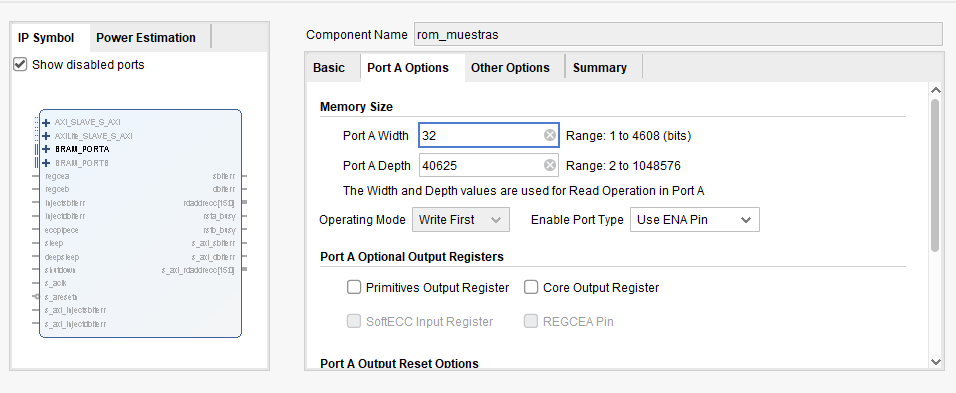
\includegraphics[width=0.6\textwidth]{./Images/img_implementacion_hw/inputromconf.png}
    \caption{Se establece la profundidad y la anchura de palabra de ROM encargada de almacenar los valores de la señal original}
    \label{fig:inputromconf}
\end{figure}
 Es importante desactivar la opción de \textit{primitive output} para que no se añada un registro extra 
 al principio y la simulación se ejecute en cada tiempo correspondiente. 
\begin{figure}[h!]
    \centering
    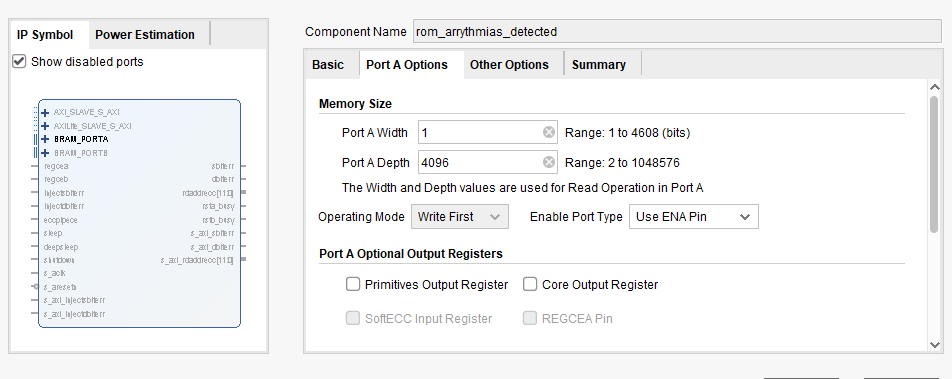
\includegraphics[width=0.6\textwidth]{./Images/img_implementacion_hw/romoutputarritmiasconf.png}
    \caption{Se establece la profundidad y la anchura de palabra de ROM encargada de almacenar el flag indicador de arritmia}
    \label{fig:romoutputarritmiasconf}
\end{figure}

\begin{figure}[h!]
    \centering
    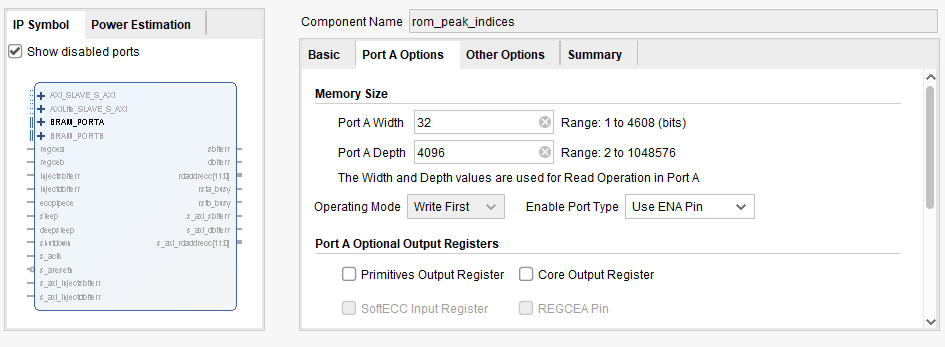
\includegraphics[width=0.6\textwidth]{./Images/img_implementacion_hw/romoutputpeakindicesconf.png}
    \caption{Se establece la profundidad y la anchura de palabra de ROM encargada de almacenar el índice de cada pico}
    \label{fig:romoutputpeakindicesconf}
\end{figure}

Para el módulo de filtrado, es necesario el uso de una ROM que contenga los coeficientes de filtrado y una RAM que contenga los valores de la señal original para ser procesados.

\begin{itemize}
\item La ROM se configura como \textit{single port ROM}, este tiene 99 filas y de anchura 
tiene 32 bits. Se muestra la configuración de este módulo en la \cref{fig:romcoeficientesconf}
\item La RAM se configura como \textit{single port RAM} y se mantiene desactivado el valor de \texttt{primitive output}.
Se muestra la configuración de este módulo en la \cref{fig:rammuestrasconf}

\end{itemize}

\begin{figure}[h!]
    \centering
    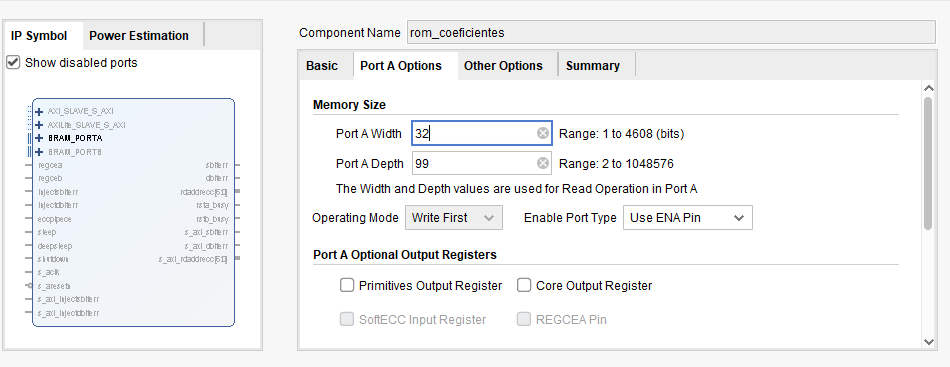
\includegraphics[width=0.6\textwidth]{./Images/img_implementacion_hw/romcoeficientesconf.png}
    \caption{Se establece la profundidad y la anchura de palabra de ROM encargada de almacenar los coeficientes}
    \label{fig:romcoeficientesconf}
\end{figure}

\begin{figure}[h!]
    \centering
    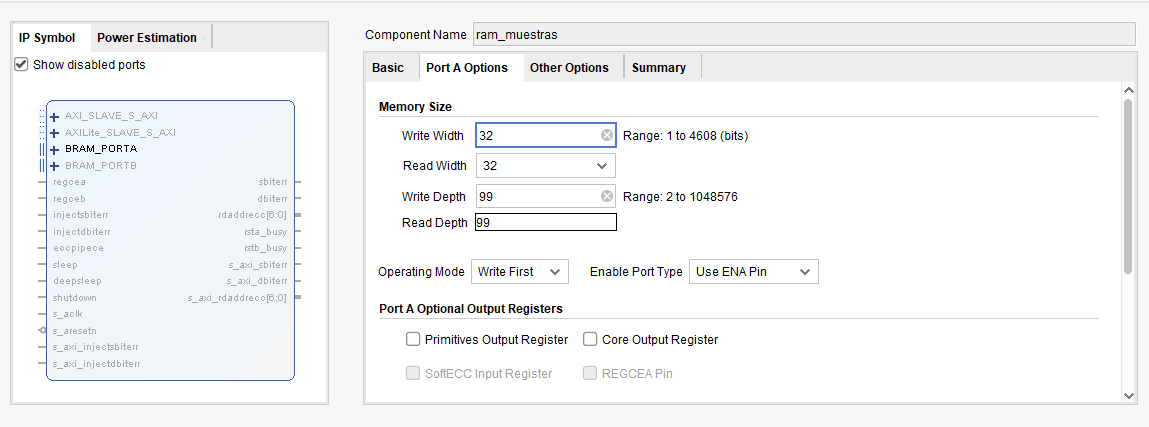
\includegraphics[width=0.6\textwidth]{./Images/img_implementacion_hw/rammuestrasconf.png}
    \caption{Se establece la profundidad y la anchura de palabra de RAM encargada de almacenar los valores de la señal original}
    \label{fig:rammuestrasconf}
\end{figure}
\FloatBarrier

\subsection{Módulos punto flotante}

Se han definido varios módulos para hacer las distintas operaciones en punto flotante, ya que en VHDL no se
pueden hacer estas operaciones directamente, se necesitan usar otros módulos especializados.

Como se operan con valores en punto flotante simple, las señales tienen que ser de 32 bits.

En este programa se necesitan 5 tipos de módulos de operaciones.

\begin{itemize}
    \item Módulo comparador mayor que: se utiliza para comparar varias señales en el módulo de detección de picos como son:
    \begin{itemize}
        \item \texttt{signal\_data gt last\_peak}
        \item \texttt{signal\_data gt cutoff}
        \item \texttt{last\_peak gt cutoff}
    \end{itemize}

    \item Módulo divisor y resta: se utilizan en conjunto para calcular el \textit{cutoff} que tiene la operación:
    \[cutoff = cutoff - cutoff/192\]

    \item Módulo multiplicación y suma: Se usa para poder multiplicar los valores de las muestras con los valores de los coeficientes en el módulo de filtrado.
    
\end{itemize}

\section{Módulo de filtrado}

\subsection{Señales de entrada y salida}

Las señales de entrada son:

\begin{itemize}
\item \texttt{clk} y \texttt{reset}.
\item \texttt{input\_signal\_data}: Señal que recibe las muestras de la señal original.
\item \texttt{input\_valid} e \texttt{input\_ready}: Flags que sirven para sincronizar el módulo con la llegada de muestras. 
\end{itemize}

Las señales de salida son:

\begin{itemize}
    \item \texttt{output\_filter\_data}: Saca los valores de la señal filtrada.
    \item \texttt{output\_filter\_index}: Saca los índices de cada valor de la señal filtrada.
    \item \texttt{output\_valid} y \texttt{output\_ready}: Sincronizan el módulo del filtrado con el módulo de detección de picos.
\end{itemize}

\begin{figure}[h!]
    \centering
    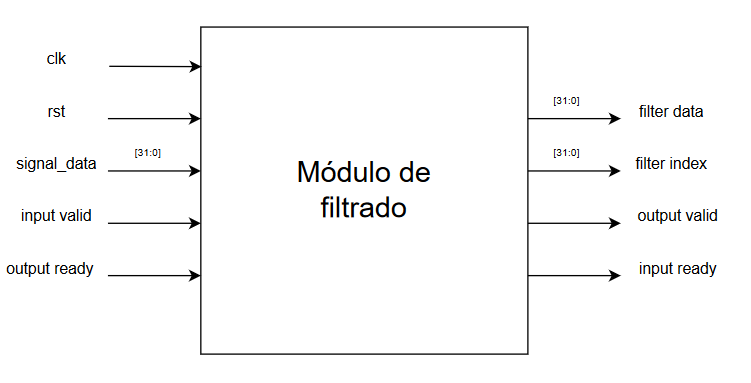
\includegraphics[width=0.6\textwidth]{./Images/img_implementacion_hw/diagramamodulofiltrado.png}
    \caption{Entradas y salidas del módulo de filtrado}
    \label{fig:modfiltrado}
\end{figure} 

\subsection{Máquina de estados}

\begin{figure}[h!]
    \centering
    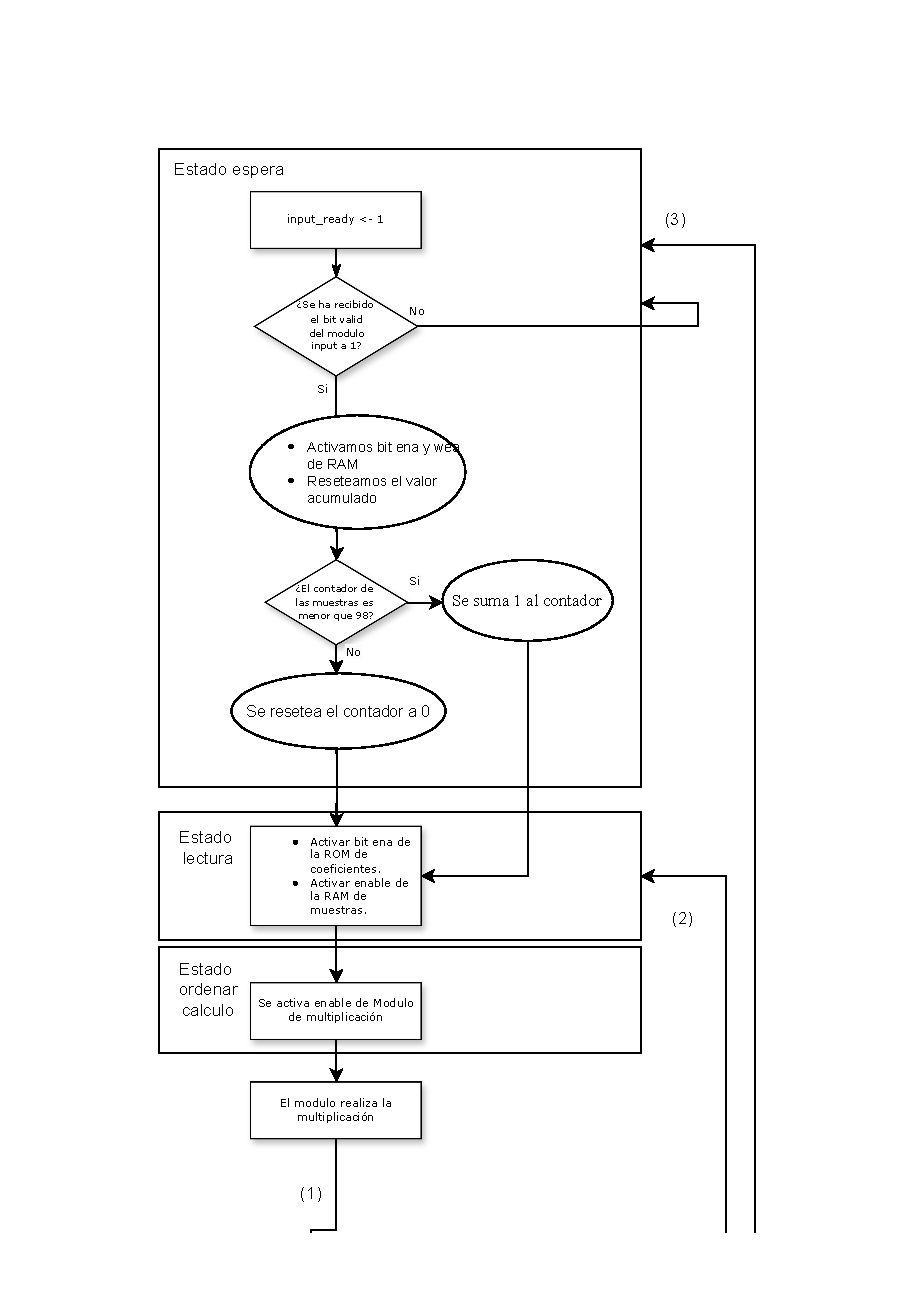
\includegraphics[width=0.99\textwidth]{./Images/img_implementacion_hw/Diagramaasmfiltrado1.pdf}
    \caption{Diagrama ASM de Módulo de filtrado de señal}
    \label{fig:Diagramaasmfiltrado1}
\end{figure} 

\begin{figure}[h!]
    \centering
    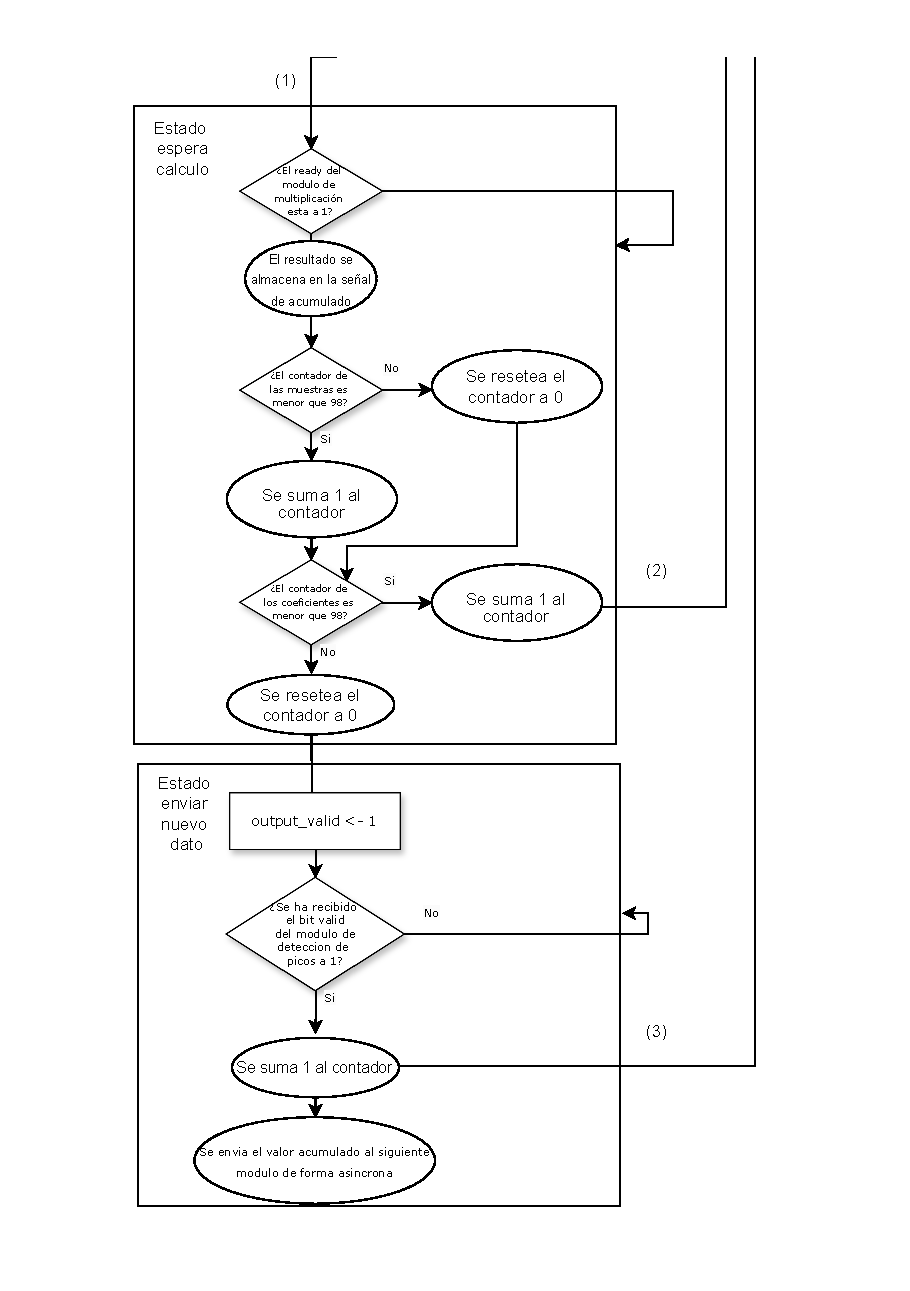
\includegraphics[width=0.99\textwidth]{./Images/img_implementacion_hw/Diagramaasmfiltrado2.pdf}
    \caption{Diagrama ASM de Módulo de filtrado de señal}
    \label{fig:Diagramaasmfiltrado2}
\end{figure} 
\FloatBarrier
El envío de datos al output se realiza de forma combinacional, se pasa a \texttt{output\_data} el 
valor del acumulado y el índice a su respectivo output.
\begin{itemize}
    \item Estado de espera: En el estado de espera se activa la señal de \texttt{ready} y se espera a que se envíe un valor de la señal sin filtrar, después se borra el valor de la solución de la multiplicación anterior, se activan las señales de escritura de la RAM y se establece el índice donde se va a escribir la muestra.
    \item Estado de lectura: Se activa el bit de lectura de los coeficientes y de las muestras.
    \item Estado para ordenar el cálculo: Se activa el flag del módulo de multiplicación y suma.
    \item Estado de espera del cálculo: Espera a que termine el módulo de multiplicación y suma esperando la señal de \texttt{ready\_muladd}
    y se almacena el resultado, también se actualiza el contador de los coeficientes, de las muestras y dependiendo de si el 
    índice de coeficientes es menor de 98, se va al estado de lectura o el estado de enviar un nuevo dato al siguiente módulo.
    \item Estado de envío de nuevo dato: Este estado sincroniza el siguiente módulo, activando así el bit de \texttt{valid} a 1 y esperando el bit
    de \texttt{ready} del siguiente módulo para poder enviar el valor filtrado.
\end{itemize}

\subsection{Módulos utilizados}
El módulo de memoria ROM que almacena los coeficientes devuelve el valor almacenado en la posición de memoria correspondiente al índice proporcionado. Además, tiene un funcionamiento circular: al llegar al índice 99, el siguiente índice será 0. Su diagrama está representado en la \cref{fig:diagramamoduloROM}.

\begin{figure}[h!]
    \centering
    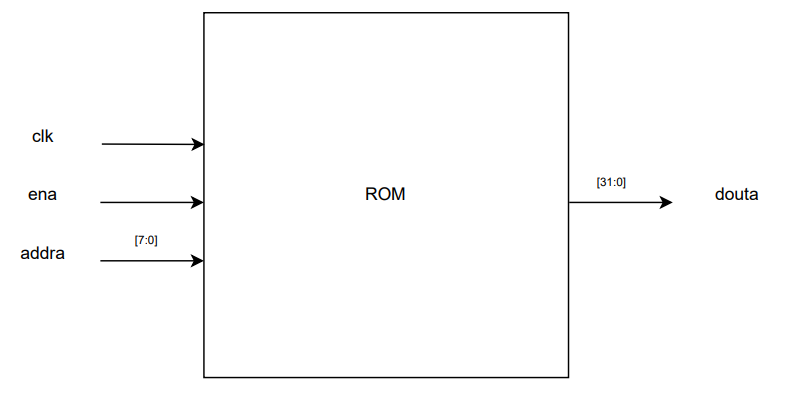
\includegraphics[width=0.6\textwidth]{./Images/img_implementacion_hw/diagramamoduloROM.png}
    \caption{Diagrama de la ROM que se usa en el filtrado de la señal}
    \label{fig:diagramamoduloROM}
\end{figure} 
\FloatBarrier

El módulo de la memoria RAM, se encarga de almacenar los valores de la señal original y posteriormente de escribir los resultados del módulo de multiplicación y suma. Este también tiene un funcionamiento circular y su diagrama se representa en la \cref{fig:diagramamoduloRAM}.

\begin{figure}[h!]
    \centering
    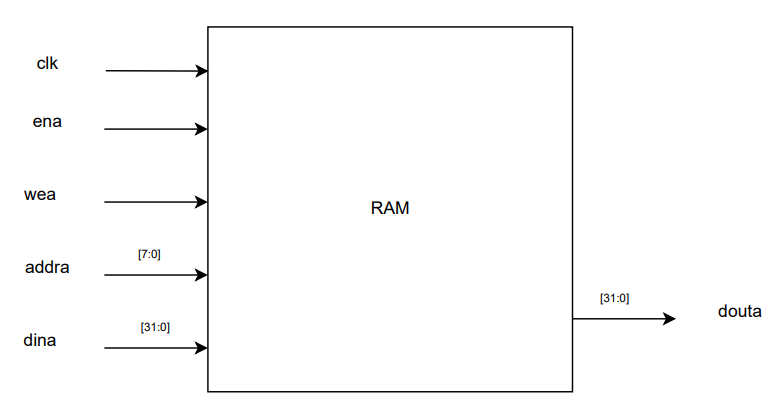
\includegraphics[width=0.6\textwidth]{./Images/img_implementacion_hw/diagramamoduloRAM.png}
    \caption{Diagrama de la RAM que se usa en el filtrado de la señal}
    \label{fig:diagramamoduloRAM}
\end{figure} 
\FloatBarrier

El módulo de multiplicación y suma de números en punto flotante se encarga de multiplicar el valor del coeficiente con el valor de la señal correspondiente y al terminar, lo suma a los valores acumulados. Su diagrama se puede ver en la \cref{fig:diagramamodulomultiplicacionysuma}.
\begin{figure}[h!]
    \centering
    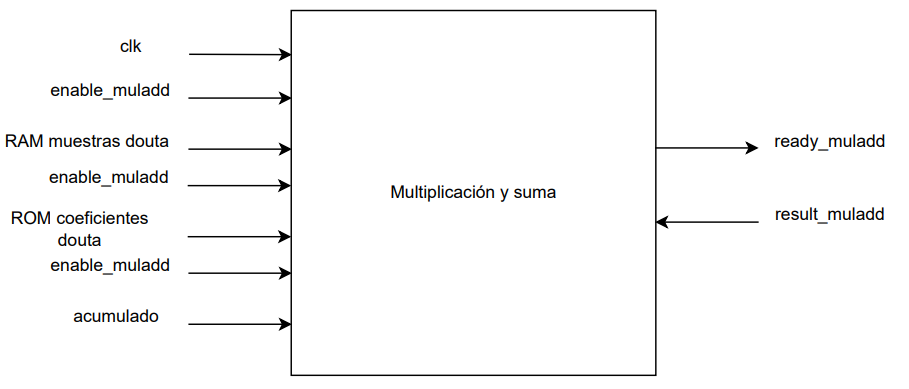
\includegraphics[width=0.9\textwidth]{./Images/img_implementacion_hw/diagramamodulomultiplicacionysuma.png}
    \caption{Diagrama de Módulo de multiplicación y suma.}
    \label{fig:diagramamodulomultiplicacionysuma}
\end{figure}
\FloatBarrier
\section{Módulo de detección de picos}

Este módulo se encarga de detectar los picos QRS de la señal filtrada.
\subsection{Señales de entrada y salida}

    \begin{figure}[h!]
        \centering
        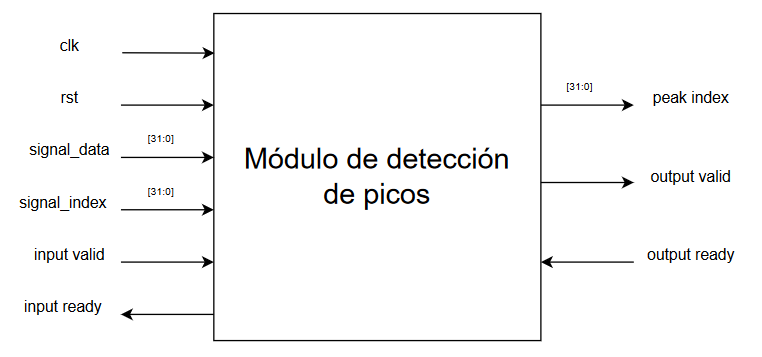
\includegraphics[width=0.6\textwidth]{./Images/img_implementacion_hw/diagramamodulodeteccionpicos.png}
        \caption{Entradas y salidas del módulo de detección de picos}
        \label{fig:moddeteccionpicos}
    \end{figure} 
    
    \begin{itemize}
    \item \texttt{clk} y \texttt{reset}.
    \item \texttt{input\_signal\_data}: señal que recibe las muestras de la señal filtrada.
    \item \texttt{input\_signal\_index}: señal que recibe los índices de las muestras de la señal filtrada.
    \item \texttt{input\_valid} e \texttt{input\_ready}: son flags que sirven para sincronizar el módulo con la llegada de muestras. 
    \end{itemize}
    
    Las señales de salida son:
    
    \begin{itemize}
        \item \texttt{output\_peak\_index}: saca los índices de los picos detectados.
        \item \texttt{output\_valid} y \texttt{output\_ready}: Se encargan de sincronizar el módulo de detección de picos 
        con el módulo de detección de arritmias.
    \end{itemize}

\subsection{Máquina de estados}

\begin{itemize}
    \item Estado de espera: En este estado, se activa la señal de \texttt{ready} y se espera a que se envíe un valor desde el módulo de filtrado.
    \item Estado de comprobar índice:
    \begin{itemize}
        \item Si no hay un pico (es decir, si la señal \texttt{last\_peak} está en 0), se asigna el valor a la señal y se registra el índice. Luego, se pasa al estado de actualizar el \textit{cutoff}, activando la señal de división para que los módulos de división y resta de valores en punto flotante comiencen a calcular el nuevo valor del \textit{cutoff}.
        \item Si hay un pico, se ordena la comparación \texttt{signal\_data > last\_peak} pasando las señales correspondientes al módulo de comparación en punto flotante. Además, se anticipa y se realiza la comparación \texttt{last\_peak > cutoff} para, en caso de que la condición anterior no se cumpla, tener esta comparación lista y poder pasar directamente al siguiente estado. También se activan las señales del módulo de comparación correspondiente. El siguiente estado es el de espera a la condición en la que la señal es mayor que el pico máximo.
    \end{itemize}
    
    \item Estado de actualizar \textit{cutoff}: 
    \begin{itemize}
        \item En este estado se espera la señal \texttt{ready} del módulo de resta, ya que es la última operación necesaria para calcular el \textit{cutoff}. Primero se ejecuta el módulo de división para calcular \texttt{cutoff/192} y luego la resta \texttt{cutoff - cutoff/192}. Cuando la señal \texttt{ready\_sub} esté en '1', se actualiza el \textit{cutoff} y se pasa al estado de espera, terminando así la iteración.
    \end{itemize}

    \item Estado de espera a la condición en la que la señal es mayor que el pico máximo: 
    \begin{itemize}
        \item Cuando las señales \texttt{ready} de los comparadores estén en '1', se podrán ejecutar las funcionalidades de este estado, el cual tiene tres condiciones:
        \begin{itemize}
            \item Si se ha encontrado un valor mayor que \texttt{last\_peak}, este valor se convierte en el nuevo \texttt{last\_peak} y el nuevo \textit{cutoff}; además, se actualiza el índice. 
            \item La señal que indica la condición de si han pasado 72 picos sin haber encontrado un pico superior se calcula de forma combinacional. Si se cumplen las condiciones de que han pasado 72 muestras sin encontrar un valor mayor que \texttt{last\_peak} y que \texttt{last\_peak} es mayor que el \textit{cutoff}, se pasa directamente al estado de envío de nuevo pico para enviar el pico QRS.
            \item Si ninguna de las condiciones anteriores se cumple, simplemente se ordena la actualización del \textit{cutoff} activando el \texttt{enable} del módulo de división y se pasa al estado correspondiente.
        \end{itemize}
    \end{itemize}
    \item Estado de envío de nuevo pico:
    \begin{itemize}
        \item En este estado, se activa la señal de \texttt{valid} a '1' y se espera a que el módulo de detección de arritmias envíe la señal de \texttt{ready}. Luego, se reinician las señales de \texttt{last\_peak} y \texttt{last\_index} a '0' y se actualiza el \textit{cutoff}.
    \end{itemize}
\end{itemize}

\begin{figure}[h!]
    \centering
    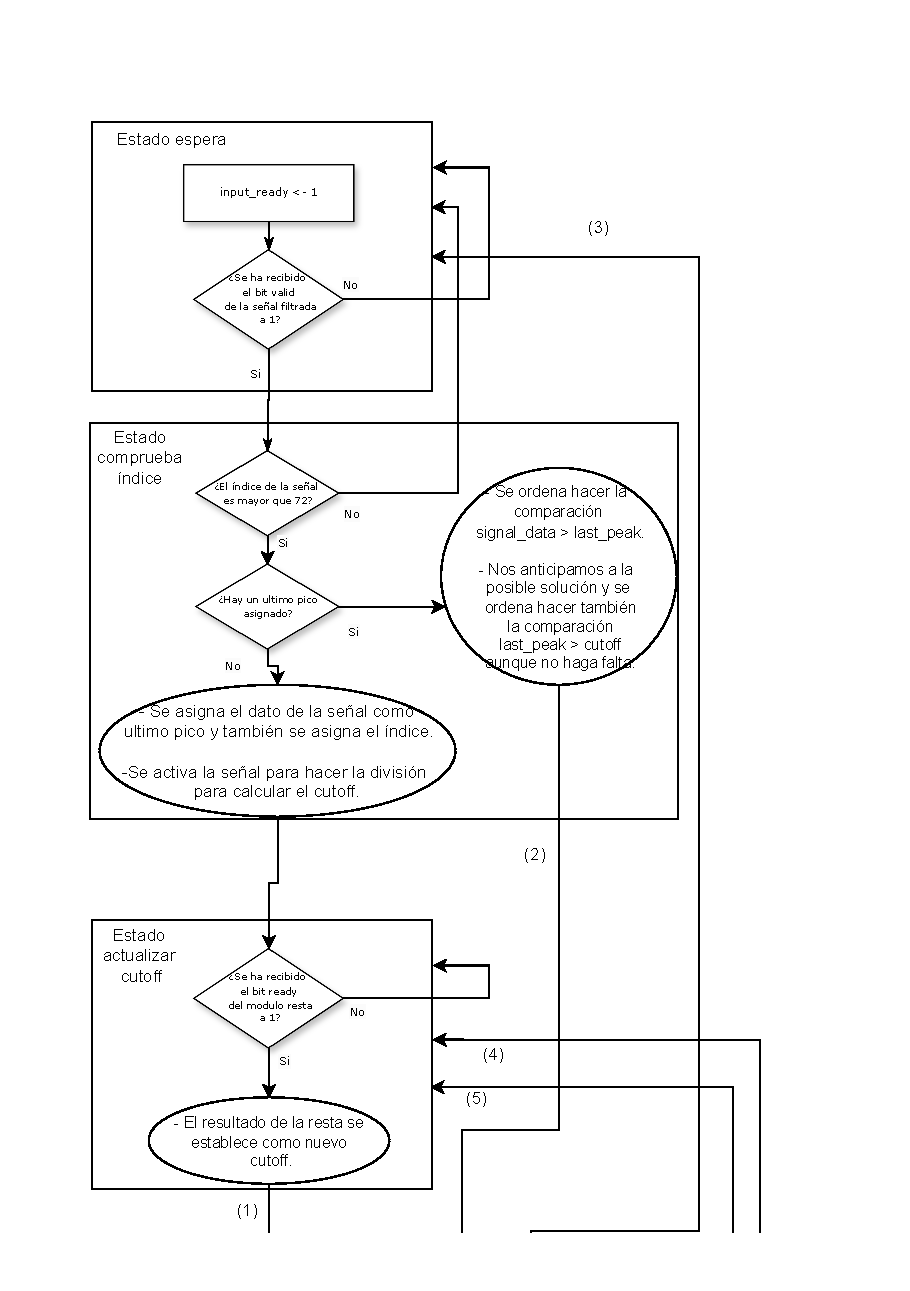
\includegraphics[width=0.99\textwidth]{./Images/img_implementacion_hw/Diagramaasmpicos1.pdf}
    \caption{Diagrama ASM de Módulo de detección de picos}
    \label{fig:Diagramaasmpicos1}
\end{figure} 

\begin{figure}[h!]
    \centering
    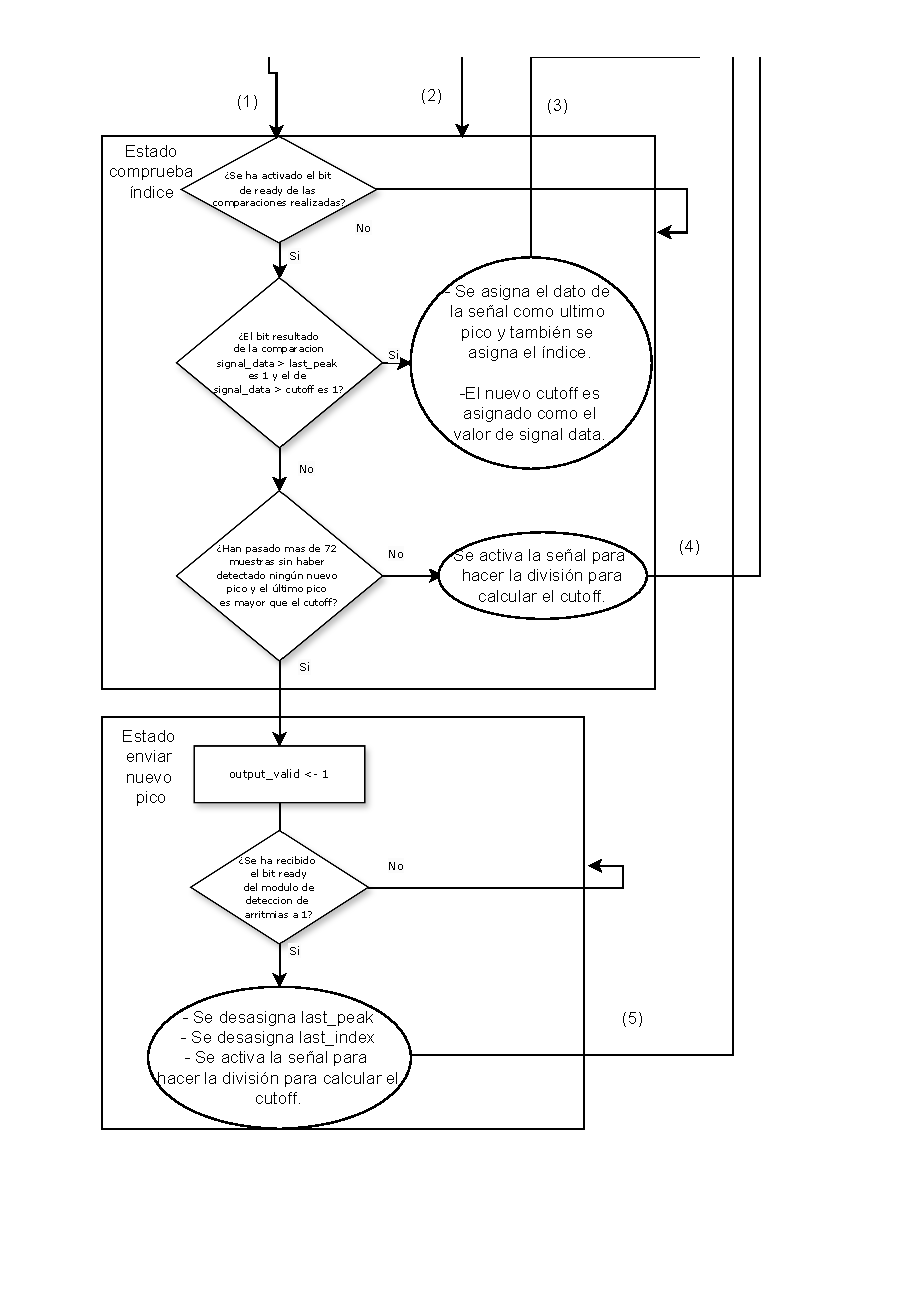
\includegraphics[width=0.99\textwidth]{./Images/img_implementacion_hw/Diagramaasmpicos2.pdf}
    \caption{Diagrama ASM de Módulo de detección de picos}
    \label{fig:Diagramaasmpicos2}
\end{figure} 
\FloatBarrier
De manera combinacional se pasa como output last index pero el módulo de detección de arritmias se activa cuando input\_valid
se activa usando así el \texttt{last\_index} correspondiente.

\subsection{Módulos utilizados}

\begin{figure}[h!]
    \centering
    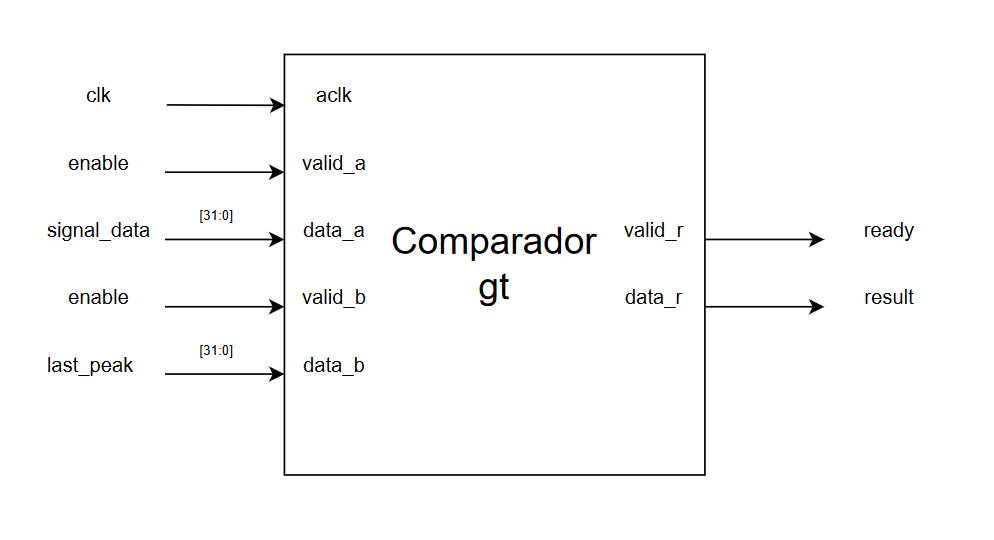
\includegraphics[width=0.8\textwidth]{./Images/img_implementacion_hw/comparadorgt.png}
    \caption{Entrada y salida del módulo de comparador}
    \label{fig:comparadorgt}
\end{figure}

\begin{figure}[h!]
    \centering
    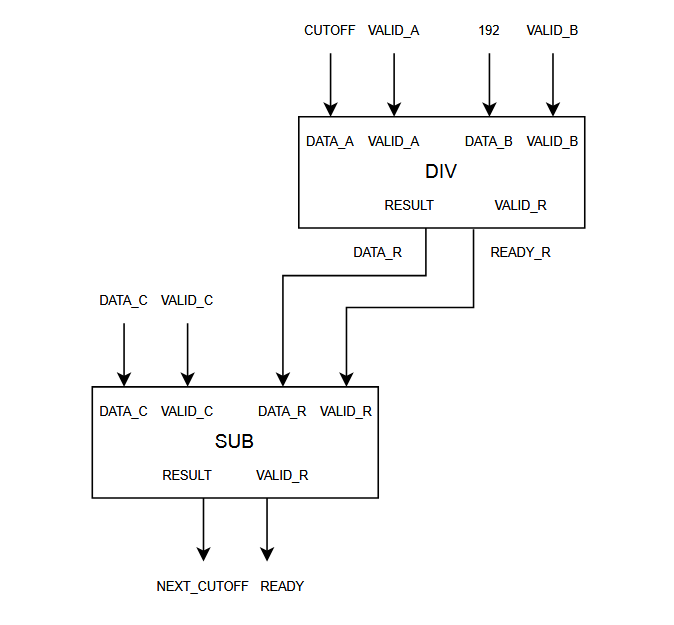
\includegraphics[width=0.6\textwidth]{./Images/img_implementacion_hw/DiagramaDivisorrestador.png}
    \caption{Funcionamiento de la conexión de los módulos de divisor y restador}
    \label{fig:divisorrestador}
\end{figure}

\section{Módulo de detección de arritmias}

El módulo de detección de arritmias se encarga de detectar si la distancia entre 2 picos QRS es considerada una arritmia o no,
 
\subsection{Señales de entrada y salida}
Las señales de entrada de este módulo son:

\begin{itemize}
    \item \texttt{clk} y \texttt{reset}.
    \item \texttt{input\_peak\_index}: señal que recibe las muestras de los picos QRS.
    \item \texttt{input\_valid} e \texttt{input\_ready}: son \textit{flags} que sirven para sincronizar este módulo con el módulo de detección de picos. 
\end{itemize}
    
Las señales de salida son:

\begin{itemize}
    \item \texttt{output\_arrythmia\_detected}: flag que saca 0 si el ritmo es normal y 1 si se ha detectado una arritmia.
    \item \texttt{output\_arrythmia\_index}: valor que indica en que \textit{sample} se ha producido la arritmia.
    \item \texttt{output\_valid} y \texttt{output\_ready}: para la sincronización con el módulo \textit{output}.
\end{itemize}

\begin{figure}[h!]
    \centering
    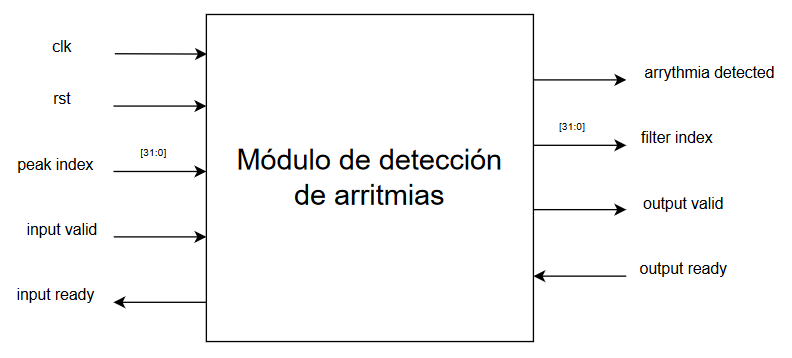
\includegraphics[width=0.6\textwidth]{./Images/img_implementacion_hw/diagramamodulodeteccionarritmias.png}
    \caption{Entradas y salidas del módulo de detección de arritmias}
    \label{fig:moddeteccionarritmias}
\end{figure} 

\subsection{Máquina de estados}

\begin{itemize}
    \item Estado de espera: En este estado se activa la señal de \textit{ready} y se espera a que se envíe un pico QRS. Después, se pasa al estado de hallar primera distancia.
    \item Estado hallar primera distancia: 
    \begin{itemize}
        \item Si el contador es 0 significa que se recibe el primer pico registrado por lo que se guarda para más tarde y se pasa al estado de espera.
        \item Si el contador es 1 significa que se recibe el segundo pico y por tanto se compara con el anterior hallando la primera distancia después pasa al estado de calcular distancia actual.
        \item Si no se cumple ninguna condición se pasa al estado de calcular distancia actual.   
    \end{itemize}
    \item Estado de calcular distancia actual: Se incrementa el contador en 1 y se calcula la distancia actual.
    \item Estado actualización de buffer: Se actualizan las variables que crean un buffer ficticio, moviendo los valores una posición cuando se añade la distancia actual, similar al funcionamiento de una cola.
    \item Estado compara distancia actual: 
    \begin{itemize}
        \item Según lo explicado en la implementación del algoritmo, la señal \texttt{TNRange} simboliza la distancia entre el pico detectado como arritmia y el pico normal actual. Este flag se activa cuando se ha detectado una arritmia, ya que \texttt{last\_distance} puede ser mayor de lo normal.
        \item Para calcular el  \textit{gap} , cuando el flag de \texttt{TNRange} está activo y el de arritmia detectada no lo está, se compara la distancia actual con la distancia de hace tres ciclos (\texttt{last\_distance - 3}).
        \item Si esta condición no se cumple, el gap se calcula comparando con la \texttt{last\_distance}.
        \item Además, si la distancia anterior correspondía a una arritmia, se desactiva el flag de arritmia detectada.
    \end{itemize}

    \item Estado procesa porcentaje: 
    \begin{itemize}
        \item Se calcula el porcentaje de forma combinacional. Si el flag de porcentaje es igual a 1, significa que el porcentaje calculado es mayor de lo esperado, por lo que se activan las flags de \texttt{TNRange} y \texttt{counter\_arrhythmias}.
        \item Independientemente de las flags, el índice y la distancia actual se actualizan a \texttt{last\_distance} y \texttt{last\_index}.
    \end{itemize}
    \item Estado envío bit: Se activa la señal de \textit{valid} y se espera a la señal de \textit{ready} para enviar el dato al módulo de salida.
\end{itemize}

Además, se calcula el porcentaje del  \textit{gap}  entre las 2 distancias con una distancia normal de forma combinacional.

\begin{itemize}
    \item Estas señales están en complemento a 2, por lo que cuando los números son negativos, el bit más significativo se cambia a 1. Dado que solo se consideran los números positivos, solo se toman en cuenta los números cuyo bit más significativo sea 0.
    \item Al inicio, la señal de la última distancia es x"00000000". Al comparar esta distancia con la actual, el resultado será una distancia muy grande que activará el bit del porcentaje calculado de forma combinacional. Este caso específico se ignora en las comparaciones.
    \item En lugar de dividir el  \textit{gap}  entre \texttt{distance\_for\_calc},  siendo g =  \textit{gap}  y d = \texttt{distance\_for\_calc}, se utiliza la siguiente fórmula:
    \[ g/d > 0.15\] 
    \[g > 0.15 \cdot d \] 
    \[g > d>> 5 + d>> 3 + d\] 
\end{itemize}

\begin{figure}[h!]
    \centering
    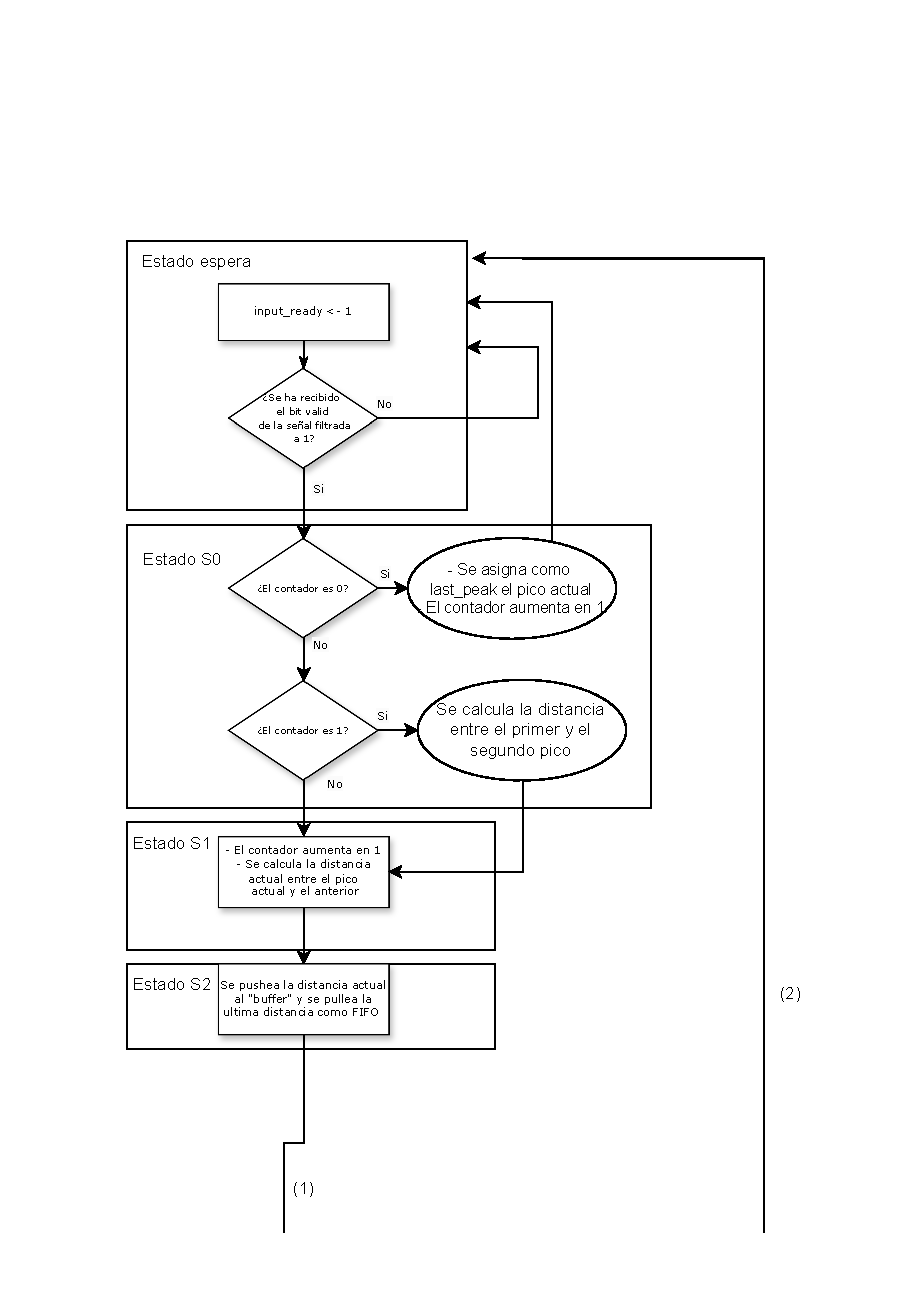
\includegraphics[width=0.99\textwidth]{./Images/img_implementacion_hw/Diagramaasmarritmias1.pdf}
    \caption{Diagrama ASM de Módulo de filtrado de señal}
    \label{fig:Diagramaasmarritmias1}
\end{figure} 

\begin{figure}[h!]
    \centering
    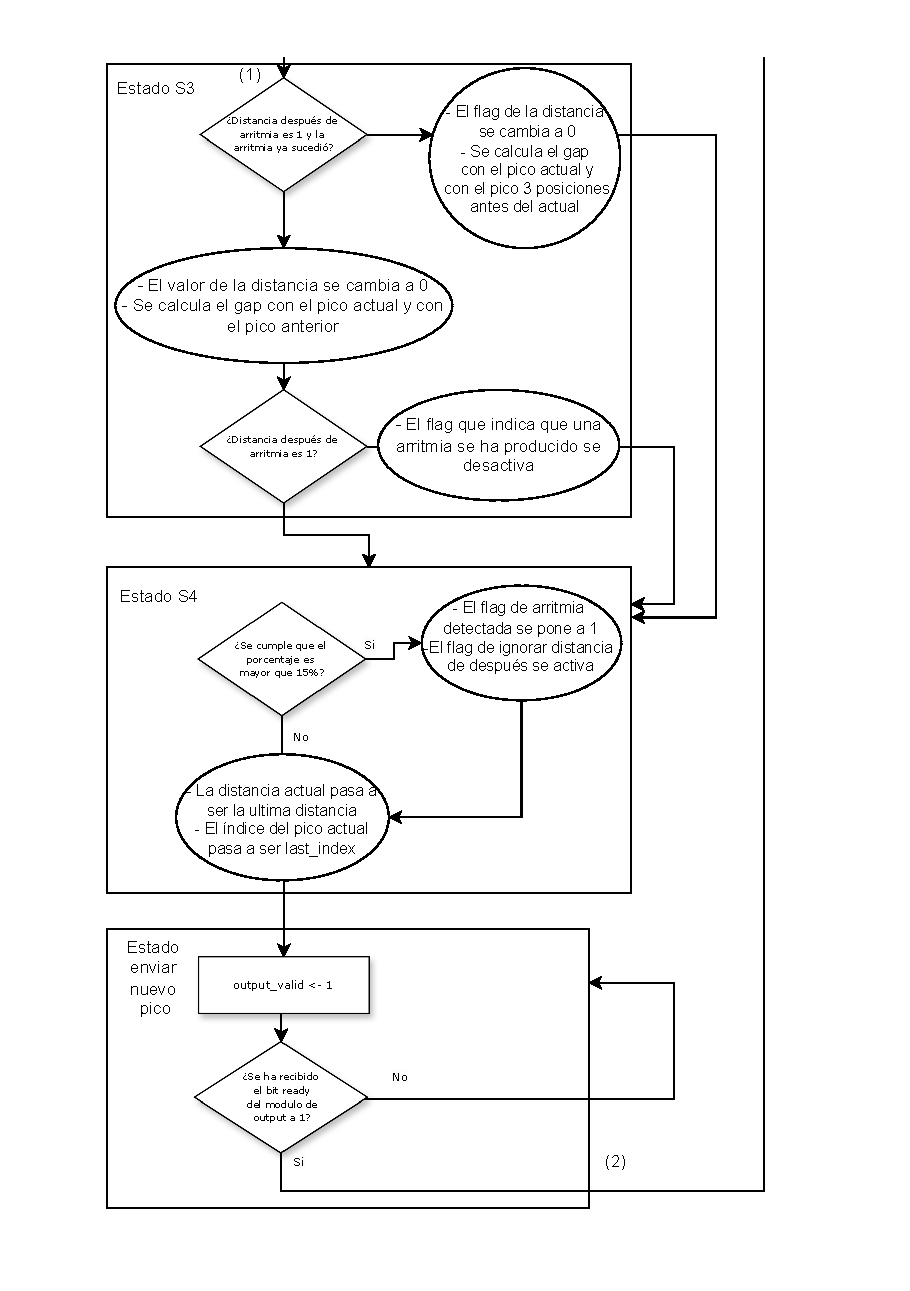
\includegraphics[width=0.99\textwidth]{./Images/img_implementacion_hw/Diagramaasmarritmias2.pdf}
    \caption{Diagrama ASM de Módulo de filtrado de señal}
    \label{fig:Diagramaasmarritmias2}
\end{figure} 
\FloatBarrier
\section{Módulos input y output}
Estos módulos se componen de un estado de lectura y uno de escritura. Uno lee el dato y el otro se encarga de esperar a que se lea el dato y actualizar el contador para que se pueda leer de la siguiente posición de la ROM.

\subsection{Módulo de entrada}
\begin{itemize}
\item Estado de lectura: Primero, se asegura de que el contador no ha llegado a la cantidad máxima de muestras, que en este caso es 40,625. Luego, se actualiza el bit de \textit{enable} a 1 y se pasa al estado de espera.
\item Estado de espera: Pone el bit de \textit{valid} a 1 y espera al bit de \textit{ready} para que el siguiente módulo lea el dato, actualiza el contador y pasa al estado de lectura.
\end{itemize}

Este módulo cuenta con una ROM con los valores de la señal original, valores que se van leyendo cundo la señal de \textit{ready} se activa.

\subsection{Módulo de salida}
\begin{itemize}
\item Estado de lectura: Primero, se asegura de que el contador no ha llegado a la cantidad máxima de muestras, que en este caso es 144. Luego, se pone el bit de enable a 1 y se pasa al estado de espera. Si se han leído todas las muestras, pasa al estado correcto.
\item Estado de espera: Pone el bit de \textit{valid} a 1 y espera al bit de \textit{ready} para que el siguiente módulo lea el dato, actualiza el contador y se comprueba si la anotación del pico coincide con la anotación de la ROM, que es la anotación original. Además, se asegura de que la anotación pertenece al índice correcto. Si esta condición se cumple, sigue con la ejecución; de lo contrario, pasa al estado de error.
\item Estado de error: Pone la señal de error a 1 y detiene la ejecución, ya que un resultado no coincide.
\item Estado correcto: Pone la señal de correcto a 1, indicando que el programa ha sido replicado con éxito.
\end{itemize}

Este módulo cuenta con una ROM que contiene los valores de la señal original, los cuales se van leyendo cuando la señal de \textit{ready} se activa.
\section{Módulo principal y testbench}

El módulo principal se encarga de sincronizar los módulos pasando los datos de un módulo al siguiente así como la señal de \textit{valid} y transferir de vuelta la señal de \textit{ready}.

Las señales de entrada del módulo principal (main) son las señales de reloj (\texttt{clk}) y de reinicio (\texttt{reset}) y las señales de salida indican si el resultado es correcto o si hay un error.

\textbf{Módulo de Filtrado:}
\begin{itemize}
    \item Toma \texttt{sample\_data} y \texttt{sample\_valid} como entradas.
    \item Produce \texttt{filter\_data}, \texttt{filter\_index}, \texttt{filter\_valid} y \texttt{filter\_ready} como salidas.
\end{itemize}

\textbf{Módulo de Detección de Picos:}
\begin{itemize}
    \item Toma \texttt{filter\_data}, \texttt{filter\_index} y \texttt{filter\_valid} como entradas.
    \item Produce \texttt{peak\_detection\_index}, \texttt{peak\_detection\_valid} y \texttt{peak\_detection\_ready} como salidas.
\end{itemize}

\textbf{Módulo de Detección de Arritmias:}
\begin{itemize}
    \item Toma \texttt{peak\_detection\_index} y \texttt{peak\_detection\_valid} como entradas.
    \item Produce \texttt{arrythmia\_detected}, \texttt{arrythmia\_index}, \texttt{arrythmia\_valid} y \texttt{arrythmia\_ready} como salidas.
\end{itemize}

También se ha definido un \textit{testbench} para las simulaciones, donde se definen los ciclos de reloj, además del \texttt{reset} al principio de la ejecución. Como salida tiene los estados de correcto y error para ver los resultados de la ejecución.